\chapter*{Benchmarking example 1: Water flow in soil}
Currently, benchmarks are developed to test dumux-rosi against analytical solutions and results of other numerical models. They are all described in Jupyter Notebooks at \lstinline{https://github.com/RSA-benchmarks/collaborative-comparison}. Here, we describe the DuMu$^x$-implementation of the 1D benchmarks of Vanderborght et al. (2005) for water flow in soil.

\section*{The model}
We solve the Richards equation for water flow in soil. Since DuMu$^x$ is developed for multi-phase flow in porous media, it uses units of absolute pressure of wetting and non-wetting phases. In the Richards equation, we assume that the non-wetting phase (air) does not change over time and has a constant pressure of 1.0 $\times$ 10$^5$ Pa. Thus, we need to solve only the equation for the wetting phase (water). We stick to the standard DuMu$^x$ units for pressure, although in soil physics, head units are more common, in order to avoid mistakes of e.g. unconsidered hard coded constants, etc. The Richards equation thus can be written as 

\begin{equation}
\frac{\partial}{\partial t} \left(\rho_w \Phi S \right) - \nabla  \cdot \left[\rho_w \frac{\kappa}{\mu}K \left(\nabla p_w-\rho_w \mathbf{g} \right) \right] = 0,
\end{equation}
with $t$ time, $\theta$ water content, $S$ saturation, $\Phi$ porosity, $S \phi = \theta$, $\rho_w$ water density, $K$ intrinsic permeability, $\mu$ dynamic viscosity, $\kappa$ relative permeability, $\mathbf{g}$ gravitational acceleration, $p_w$ absolute pressure of wetting phase (water)\footnote{$p_w$ is the absolute pressure. The matric pressure $p_m$ is defined as $p_m = p_w-p_a$, where $p_a$ is the air pressure, assumed to be constant and equal to 1.0 $\times$ 10$^5$ Pa in this Richards equation model. In order to have head units, we need to convert the water potential from energy per unit volume of water (pressure) to energy per unit weight, i.e., $h_m=\frac{p_m}{\rho_w \mathbf{g}}$}. $\theta$ and $h_m$ are related by the water retention curve: $\theta:= \theta(h)$ (e.g. van Genuchten model).

Different initial and boundary conditions can be prescribed via the input file. Boundary conditions have number codes following (previous versions of) Hydrus: \\
constantPressure = 1,\\
constantFlux = 2, \\
atmospheric = 4, \\
freeDrainage = 5.

\section*{The input files}
Model parameters, initial and boundary conditions can be specified via the input file such that no re-building of the code is required. 
Here is the listing of the input file \lstinline{dumux-rosi/rosi_benchmarking/soil/benchmarks_1d/b1a.input}: 
\lstinputlisting[language={}, caption=input file]{dumux-rosi/rosi_benchmarking/soil/benchmarks_1d/b1a.input}	

\section*{The DuMu$^x$ code representation of model equations}
In this section, we explain where the different terms of the model equations can be found in the DuMu$^x$ code, i.e., the storage, flux and sink terms. 
The storage term is defined in the file \\
\verb+/dumux/dumux/porousmediumflow/Richards/localresidual.hh+, and is computed as\\
\lstinputlisting[firstline=91,lastline=93, language=C++, caption=Storage term]{dumux/dumux/porousmediumflow/richards/localresidual.hh}		
In this example, there is no source or sink term. 


The flux term is hidden in deeper layers of the code as part of the numerical scheme. In order to see it, we have to find out the flux type of the problem in the file 
\verb+/dumux/dumux/porousmediumflow/richards/...+. In this example, the flux type is ''darcyslaw``. Its implementation can then be found in the folder \verb+/dumux/dumux/flux+, and is then different for the different numerical schemes (e.g. cell-centered finite volume scheme with two-point flux approximation (TPFA)). 

%The file \verb+fluxvariables.hh+ in the folder \verb+/dumux/dumux/porousmediumflow/richards/+ defines the volume flux variable for the Richards equation by setting the nonwetting phase flux variable to zero. 
%\lstinputlisting[firstline=50,lastline=70, language=C++, caption=flux term b]{dumux/dumux/porousmediumflow/Richards/implicit/fluxvariables.hh}	

%The  definition for the wetting phase (water) is given in\\
%\verb+dumux/dumux/porousmediumflow/implicit/darcyfluxvariables.hh+. \\
%\lstinputlisting[firstline=19,lastline=349, language=C++, caption=flux term c]{dumux/dumux/porousmediumflow/implicit/darcyfluxvariables.hh}	

%The sink term is defined in the file\\ 
%\verb+dumux-rosi/rosi_examples/richardsrootsystem/richardstestproblem.hh+.\\
%\lstinputlisting[firstline=245,lastline=265, language=C++, caption=sink term]{dumux-rosi/rosi_examples/richardsrootsystem/richardstestproblem.hh}	

The implementation of the boundary conditions specified in the input file are implemented in the file\\ 
\verb+ dumux-rosi/rosi_benchmarking/soil/richardsproblem.hh+.\\
\lstinputlisting[firstline=188,lastline=224, language=C++, caption=Boundary conditions]{dumux-rosi/rosi_benchmarking/soil/richardsproblem.hh},
%
\lstinputlisting[firstline=229,lastline=252, language=C++, caption=Boundary conditions]{dumux-rosi/rosi_benchmarking/soil/richardsproblem.hh}	
and
\lstinputlisting[firstline=257,lastline=334, language=C++, caption=Boundary conditions]{dumux-rosi/rosi_benchmarking/soil/richardsproblem.hh}.		
											

\section*{Results}
The vtk output of 3D simulations may be visualised using Paraview. In this case, we only have a 1D simulation, therefore, we do the visualisation after postprocessing in Python. 

\begin{figure}[ht]
	\centering
  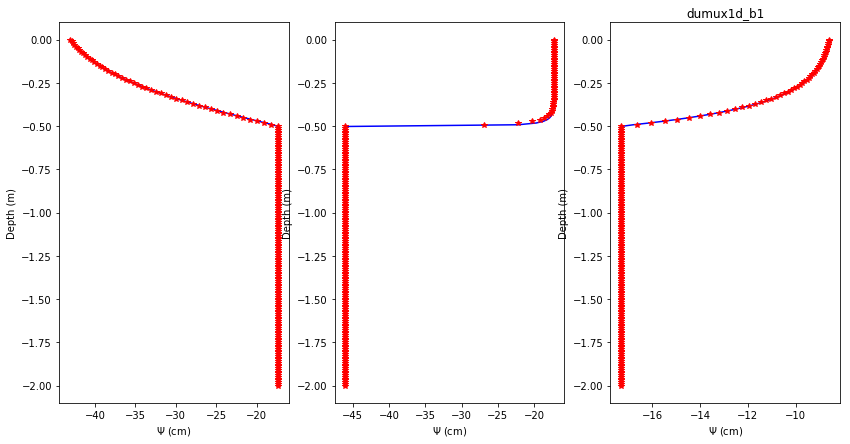
\includegraphics[width=1\textwidth]{benchmark1.png}
	\captionsetup{labelformat=empty}
	\caption{Results of benchmark problem 1. Blue: analytical solution, Red: numerical solution by DuMu$^x$}
	%\label{RWU}
\end{figure}

